%-------------------------
% Ramit Sharma - CV
% LaTeX Template
%-------------------------

\documentclass[11pt,a4paper]{article}

% Packages
\usepackage[utf8]{inputenc}
\usepackage[T1]{fontenc}
\usepackage[margin=0.75in]{geometry}
\usepackage{titlesec}
\usepackage{enumitem}
\usepackage{hyperref}
\usepackage{xcolor}
\usepackage{fontawesome5}
\usepackage{graphicx}
\usepackage{tabularx}
\usepackage{array}
\usepackage{multicol}
\usepackage{tikz}
\usepackage{parskip}

% Colors
\definecolor{primaryblue}{HTML}{2563EB}
\definecolor{darkgray}{HTML}{374151}
\definecolor{lightgray}{HTML}{6B7280}
\definecolor{verylightgray}{HTML}{E5E7EB}

% Hyperlink setup
\hypersetup{
    colorlinks=true,
    linkcolor=primaryblue,
    urlcolor=primaryblue,
    pdftitle={Ramit Sharma - CV},
    pdfauthor={Ramit Sharma}
}

% Section formatting
\titleformat{\section}
    {\Large\bfseries\color{darkgray}}
    {\faIcon{briefcase}}{0.5em}{}
    [\titlerule]

\titlespacing*{\section}{0pt}{12pt}{8pt}

% Custom commands
\newcommand{\cvheader}[6]{
    \begin{minipage}[t]{0.65\textwidth}
        {\Huge\bfseries\color{darkgray} #1}\\[4pt]
        {\large\color{primaryblue} #2}\\[10pt]
        \begin{tabular}{@{}l@{\hspace{8pt}}l@{}}
            \faIcon{linkedin} & \href{#3}{linkedin.com/in/ssramitsharma}\\[3pt]
            \faIcon{github} & \href{#4}{github.com/ssramitsharma}\\[3pt]
            \faIcon{phone} & #5\\[3pt]
            \faIcon{envelope} & \href{mailto:#6}{#6}\\[3pt]
            \faIcon{map-marker-alt} & 15-June-1991, Nepal
        \end{tabular}
    \end{minipage}%
    \hfill
    \begin{minipage}[t]{0.28\textwidth}
        \raggedleft
        \begin{tikzpicture}
            \clip (0,0) circle (2cm);
            \node at (0,0) {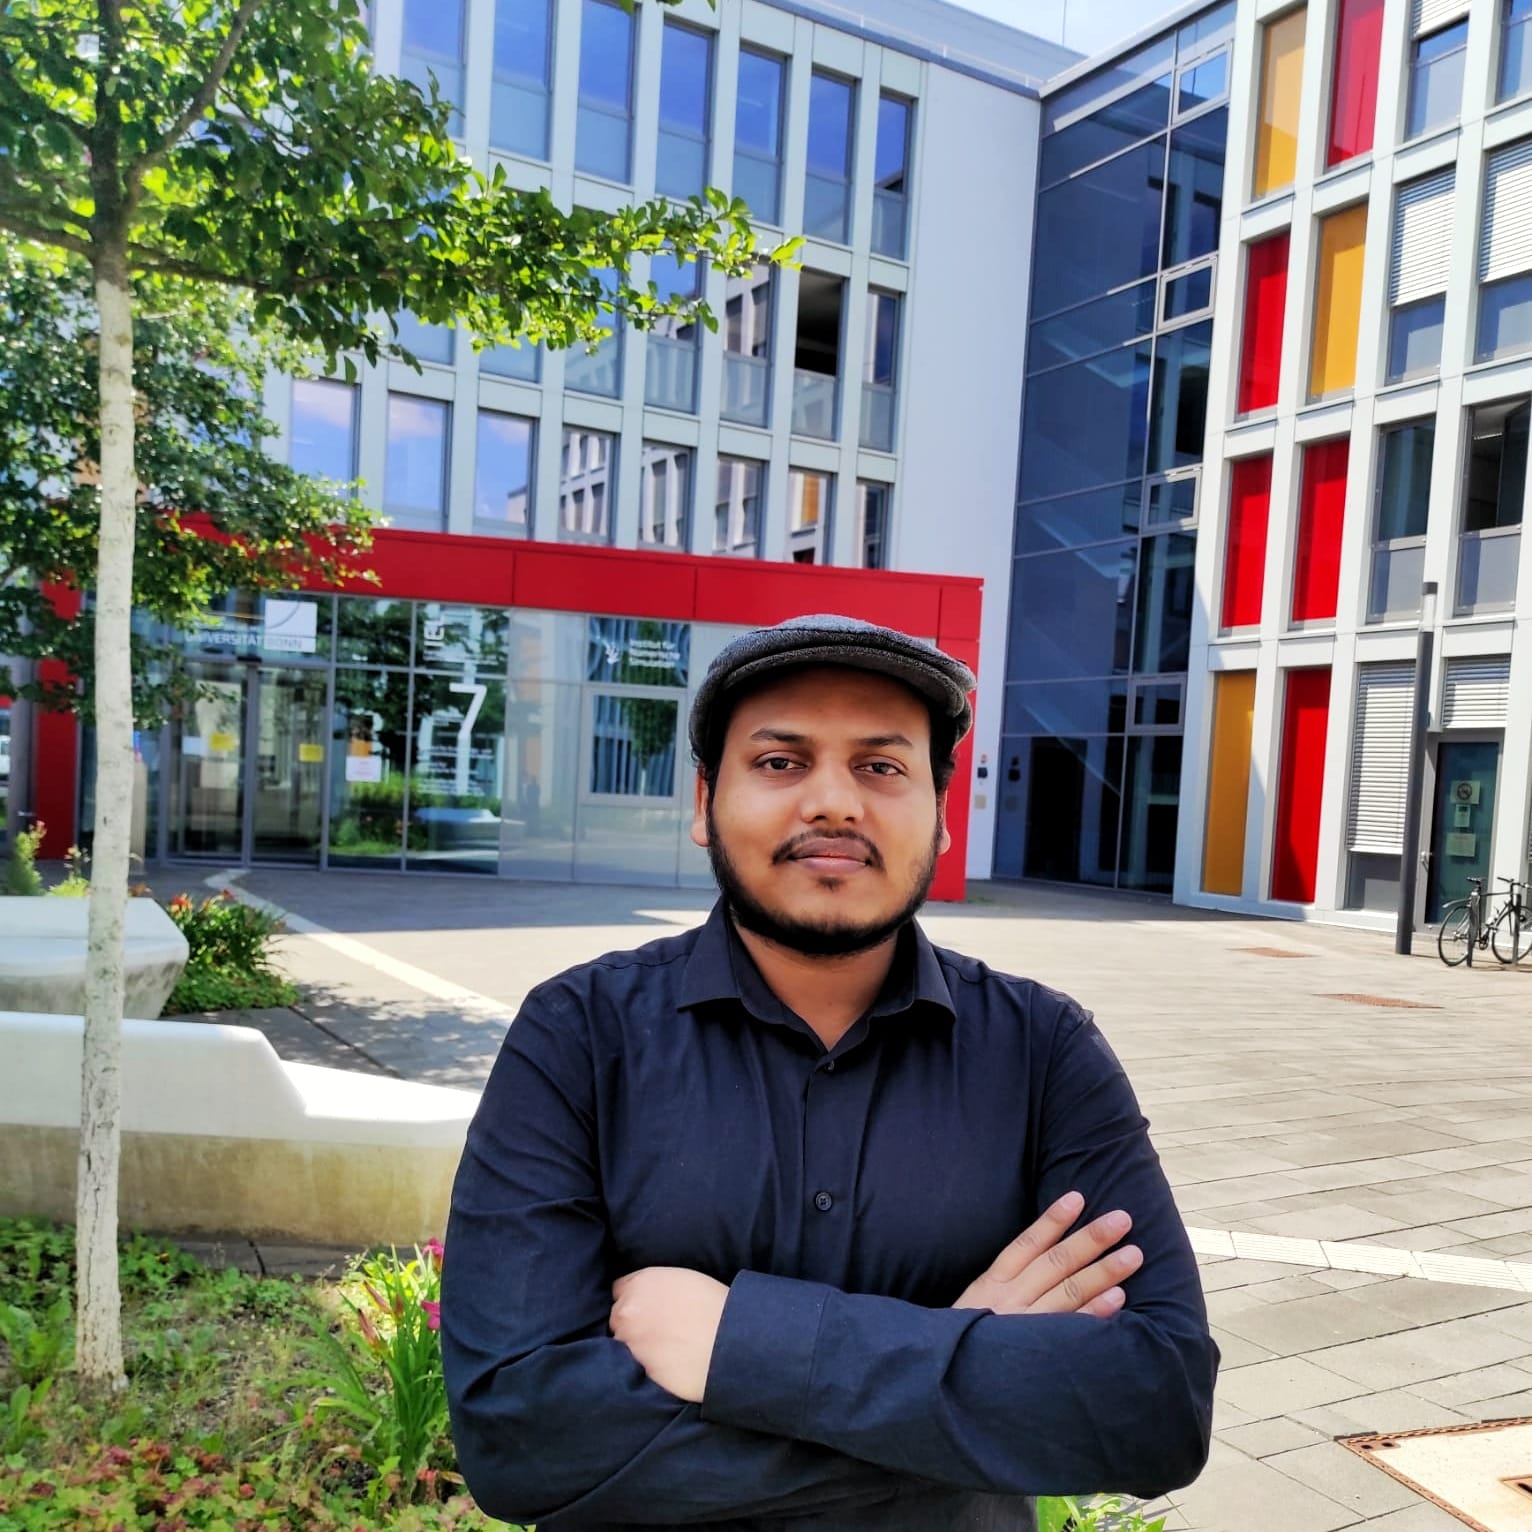
\includegraphics[width=4cm]{../assets/profile.jpg}};
        \end{tikzpicture}
    \end{minipage}
    \vspace{10pt}
}

\newcommand{\experienceitem}[5]{
    \noindent
    \begin{tabularx}{\textwidth}{@{}X r@{}}
        \textbf{#1}, \textsc{#2}, #3 & \textcolor{lightgray}{#4}
    \end{tabularx}
    \begin{itemize}[leftmargin=15pt, topsep=2pt, itemsep=1pt, parsep=0pt]
        #5
    \end{itemize}
    \vspace{2pt}
    \noindent\textcolor{verylightgray}{\rule{\textwidth}{0.5pt}}
    \vspace{6pt}
}

\newcommand{\experienceitemwithskills}[6]{
    \noindent
    \begin{tabularx}{\textwidth}{@{}X r@{}}
        \textbf{#1}, \textsc{#2}, #3 & \textcolor{lightgray}{#4}
    \end{tabularx}
    \begin{itemize}[leftmargin=15pt, topsep=2pt, itemsep=1pt, parsep=0pt]
        #5
    \end{itemize}
    \vspace{4pt}
    \noindent\fcolorbox{verylightgray}{white}{\parbox{\dimexpr\textwidth-2\fboxsep-2\fboxrule}{
        \footnotesize\textcolor{lightgray}{#6}
    }}
    \vspace{8pt}
}

\newcommand{\educationitem}[5]{
    \noindent
    \begin{tabularx}{\textwidth}{@{}X r@{}}
        \textbf{#1} & \textcolor{lightgray}{#2}\\
        \textsc{#3}, #4 &
    \end{tabularx}
    \begin{itemize}[leftmargin=15pt, topsep=2pt, itemsep=1pt, parsep=0pt]
        #5
    \end{itemize}
    \vspace{6pt}
}

\newcommand{\skillcategory}[2]{
    \noindent\textbf{#1:} #2\\[4pt]
}

% Language proficiency dots
\newcommand{\languagedots}[1]{%
    \foreach \i in {1,...,5}{%
        \ifnum\i>#1
            \textcolor{verylightgray}{\faIcon{circle}}%
        \else
            \textcolor{primaryblue}{\faIcon[solid]{circle}}%
        \fi
        \hspace{1pt}%
    }%
}

%-------------------------
% Document Start
%-------------------------
\begin{document}

\pagestyle{empty}

%-------------------------
% Header
%-------------------------
\cvheader
    {Ramit Sharma}
    {Machine Learning Engineer}
    {https://linkedin.com/in/ssramitsharma}
    {https://github.com/ssramitsharma}
    {+49 17674545056}
    {ssramitsharma@gmail.com}

%-------------------------
% Professional Summary
%-------------------------
\\vspace{6pt}
\\noindent{\\textbf{Professional Summary}}\\\\
Machine Learning Engineer with experience building production ML systems for NLP, audio and medical imaging. Skilled in designing data pipelines, training and deploying models (LLMs, CNNs, time-series), and collaborating with cross-functional teams to deliver scalable solutions. Proven track record delivering research-to-production projects and improving model quality and inference performance.

\\vspace{8pt}

%-------------------------
% Work Experience
%-------------------------
\section*{\faIcon{briefcase} \hspace{0.3em} Work Experience}

\experienceitemwithskills
    {Machine Learning Research Engineer}
    {Aaron GmbH}
    {Berlin, Germany}
    {Jun 2022 -- Dec 2023}
    {
        \item Designed and implemented data pipelines for cleaning, anonymization and feature extraction to support large-scale model training
        \item Built and validated ML models for text and audio, including preprocessing, augmentation and evaluation pipelines
        \item Improved dialogue flow and user experience through model-driven enhancements and offline/online evaluation
    }
    {Python \textbar{} TensorFlow \textbar{} Keras \textbar{} PyTorch \textbar{} Pandas \textbar{} Librosa \textbar{} NumPy \textbar{} Scikit-learn \textbar{} Flair \textbar{} Whisper \textbar{} regex \textbar{} AWS Sagemaker \textbar{} AWS Athena \textbar{} AWS Glue \textbar{} Jira \textbar{} Bitbucket \textbar{} ChatGPT}

\experienceitemwithskills
    {Research Assistant}
    {Fraunhofer IAIS}
    {Sankt Augustin, Germany}
    {Oct 2020 -- Sep 2021}
    {
        \item Developed lesion detection methods for 3D CT volumes and implemented repeatable model evaluation pipelines
        \item Trained and benchmarked object detection models (RetinaNet, YOLOv3, YOLOv5) across multiple resolutions; documented accuracy vs.\ speed trade-offs and improvement opportunities
    }
    {Python \textbar{} TensorFlow \textbar{} Keras \textbar{} PyTorch \textbar{} Pandas \textbar{} NumPy \textbar{} Scikit-learn \textbar{} Git \textbar{} GPU Cluster}

\experienceitemwithskills
    {Digitization for Industrial Engineering Intern}
    {Audi AG}
    {Ingolstadt, Germany}
    {Nov 2019 -- Apr 2020}
    {
        \item Designed software and data structures for digitization workflows in Industrial Engineering
        \item Modeled production components and implemented scenario-comparison tools to support decision making
        \item Validated and optimized tools; produced user documentation and delivered handover materials
    }
    {Python \textbar{} Pandas \textbar{} NumPy \textbar{} Tkinter \textbar{} Git \textbar{} Docker}

\experienceitemwithskills
    {Applied Machine Learning Intern}
    {Insoro GmbH}
    {Cologne, Germany}
    {Apr 2019 -- Jun 2019}
    {
        \item Applied LSTM and GRU-based models for capital markets time-series forecasting and backtesting
        \item Implemented automated test cases and evaluation scripts for portfolio optimization workflows
    }
    {Python \textbar{} TensorFlow \textbar{} Keras \textbar{} PyTorch \textbar{} Pandas \textbar{} NumPy \textbar{} Scikit-learn}

%-------------------------
% Education
%-------------------------
\section*{\faIcon{graduation-cap} \hspace{0.3em} Education}

\educationitem
    {Masters of Science in Autonomous Systems}
    {Apr 2017 -- Jan 2022}
    {Hochschule Bonn-Rhein-Sieg}
    {Sankt Augustin, Germany}
    {
        \item Studied subjects like Artificial Intelligence, Neural Networks, Learning and Adaptivity, Computer Vision, Natural Language Processing
        \item Worked on Natural Language Inference project and did a master thesis on ``Object Detection in Dense Volume Data''
    }

\educationitem
    {Bachelor of Engineering in Electrical and Electronics}
    {Aug 2010 -- Jun 2014}
    {Ramaiah Institute of Technology}
    {Bengaluru, India}
    {
        \item Thesis in Estimation of Line Parameters of standard IEEE 14 Bus system
    }

%-------------------------
% Competencies
%-------------------------
\section*{\faIcon{cogs} \hspace{0.3em} Competencies}

\skillcategory{Programming}{Python, Matlab, Java, C++, HTML, CSS}

\skillcategory{Python Libraries}{NumPy, Pandas, SciPy, Librosa, TensorFlow, Keras, PyTorch, Tkinter, Scikit-learn, Matplotlib, OpenCV, Os, PIL, Pydicom, NLTK, SpaCy, Gensim, Flask, MLflow, Flair, Whisper}

\skillcategory{Databases \& Tools}{MySQL, Sublime Text, Eclipse, Codeblocks, PyCharm, Atom, Jupyter Notebook, Spyder, Git, Docker, GPU Cluster, Heroku, AWS Sagemaker, AWS Athena, AWS Cloudwatch, Jira, ChatGPT}

\skillcategory{Operating Systems}{Windows, Linux Ubuntu, macOS}

%-------------------------
% Languages & Personal Website
%-------------------------
\vspace{8pt}
\begin{minipage}[t]{0.48\textwidth}
\section*{\faIcon{globe} \hspace{0.3em} Personal Website}
I made a personal website using HTML, CSS, and JavaScript. Hosted on GitHub Pages.\\[4pt]
\faIcon{link} \href{https://ssramitsharma.github.io}{https://ssramitsharma.github.io}
\end{minipage}%
\hfill
\begin{minipage}[t]{0.48\textwidth}
\section*{\faIcon{language} \hspace{0.3em} Languages}
\begin{tabular}{@{}l@{\hspace{12pt}}l@{}}
    English & \languagedots{5}\\[2pt]
    Hindi & \languagedots{5}\\[2pt]
    Nepali & \languagedots{4}\\[2pt]
    German & \languagedots{1}
\end{tabular}
\end{minipage}

%-------------------------
% Footer
%-------------------------
\vfill
\begin{center}
    \textcolor{lightgray}{\footnotesize Last updated: \today \hspace{10pt} | \hspace{10pt} Ramit Sharma - CV}
\end{center}

\end{document}

